% !TeX program = pdflatex
\documentclass[11pt,a4paper]{article}
\usepackage[utf8]{inputenc}
\usepackage[T1]{fontenc}
\usepackage[turkish]{babel}
\usepackage{lmodern}
\usepackage{geometry}
\usepackage{graphicx}
\usepackage{float}
\usepackage[section]{placeins}
\usepackage{flafter}
\usepackage{etoolbox}
\usepackage{caption}
\usepackage{subcaption}
\usepackage{booktabs}
\usepackage{siunitx}
\usepackage{hyperref}
\usepackage{longtable}
\usepackage{xcolor}
\usepackage{amsmath,amssymb}
\usepackage{microtype}

\geometry{margin=1.4cm}
\hypersetup{colorlinks=true,linkcolor=blue,citecolor=blue,urlcolor=blue}
% Make figure lookup robust regardless of build CWD
\graphicspath{{../results/}{results/}{./}{../}}
\DeclareGraphicsExtensions{.png,.pdf,.jpg,.jpeg}
\setkeys{Gin}{width=0.95\linewidth, keepaspectratio}
\floatplacement{figure}{H}
\floatplacement{table}{H}
\captionsetup{font=small,labelfont=bf}
% Avoid babel turkish active shorthand conflicts (e.g., '=') with URLs
\AtBeginDocument{\shorthandoff{=}}
% Ensure floats do not cross headings and appear after their definitions
\preto\section{\FloatBarrier}
\preto\subsection{\FloatBarrier}
\AfterEndEnvironment{figure}{\FloatBarrier}
\AfterEndEnvironment{table}{\FloatBarrier}
\AfterEndEnvironment{longtable}{\FloatBarrier}

\title{Yazılım Tedarik Zincirinde Kritiklik Haritalaması\\En Popüler 1000 NPM Paketinin Topolojik Risk Değerlendirmesi}
\author{\textbf{Yusuf Talha ARABACI}}
\date{Ekim 2025}

\begin{document}
\maketitle

\begin{abstract}
NPM ekosisteminde tek bir bağımlılıktaki kusur veya kötü niyetli değişiklik, transitif bağımlılıklar üzerinden geniş bir etki alanına yayılabilir. Bu bildiri, paket içeriklerinden ziyade paketler arası ilişkilerin \emph{topolojik} yapısına odaklanır. Bağımlı $\to$ bağımlılık yönünde kurulan yönlü ağ üzerinde in-degree, out-degree ve betweenness merkeziyetleri hesaplanır; bu ölçüler min–max normalizasyonu ile bir \emph{Bileşik Risk Skoru}na (BRS) dönüştürülür. Ayrıca, en kritik düğümlerin çıkartılmasıyla ağın bağlanırlılığı üzerinde bir \emph{sağlamlık} değerlendirmesi yapılır. Tüm görseller ve tablolar \texttt{results/} dizinindeki çıktılara dayanır ve ilgili başlıklar altında sunulur.
\end{abstract}

\clearpage

\section{Giriş ve Özgün Katkı}
Modern yazılım tedarik zincirinde tek bir bağımlılıktaki hata ya da kasıtlı değişiklik, transitif bağımlılıklar üzerinden yüzlerce hatta binlerce projeye yayılabilir. NPM ekosistemi; ölçek, sürüm sıklığı ve yoğun bağımlılık grafiği nedeniyle bu tür zincirleme risklere özellikle açıktır. Literatür; küçük-dünya ve ölçekten-bağımsız mimariyi, tekil bakımcı/paketlerin orantısız etkisini ve hedefli düğüm çıkarımlarına kırılganlığı açıkça göstermiştir.

Bu çalışmanın \textbf{özgün katkıları}:
\begin{itemize}
  \item Son 12 aya dayalı indirme verisiyle seçilen \textbf{Top 1000} paket üzerinde, resmî çözümleme kuralları gözetilerek kurulan yönlü graf üzerinden \textbf{Bileşik Risk Skoru (BRS)} tanımlanır ve uygulanır (in/out/betweenness + min–max + ağırlıklar: 0.5/0.2/0.3).
  \item \textbf{Kaskad etki} (ters yön dependents erişilebilirliği) ve \textbf{sağlamlık} (bileşenleşme, LCC boyutu) analizleriyle topolojik riskin sistemik etkisi nicelleştirilir.
  \item BRS, tespit hatları (Amalfi, Cerebro, OSCAR) için \textbf{öncelikli tarama kuyruğu} ve politika/bütünlük hattı (in-toto, imza benimsemesi) için \textbf{hedef paket listeleri} üretmek üzere konumlandırılır.
\end{itemize}

Kod ve özet sonuçlar: \url{https://yusufarbc.github.io/npm-complex-network-analysis/}

\section{Literatür Taraması}
Bu bölüm, \texttt{academic/LITERATURE\_REVIEW.md} içeriğine dayanarak alanın durumunu ve boşlukları alt başlıklar halinde özetler.

\subsection{Tehdit Taksonomileri ve Vaka Derlemeleri}
Backstabber’s Knife Collection gerçek saldırı örneklerinden bir taksonomi çıkarır; The Hitchhiker’s Guide ekosistemler-arası kurulum/çalışma zamanı tekniklerini sistematize eder. Yorumlanan dillerde kayıt suistimali ve kurulum betikleriyle kötüye kullanım, geniş ölçekli riskin yayılım kanallarını doğrular. NPM-odaklı fenomenler (Wyss) kurulum zamanı saldırılar, klon kodlar, meta veride oltalama gibi pratik riskleri ortaya koyar.

\subsection{Ağ-Topoloji Kırılganlığı}
Zimmermann ve Hafner, hedefli düğüm çıkarımlarında kırılganlığı; Oldnall, küçük-dünya ve ölçekten-bağımsız mimariyi ve aşırı ters-bağımlılık kapsamlarını gösterir. Bulgular, az sayıda omurga paketin orantısız sistemik etki taşıdığını ve \emph{topoloji tabanlı önceliklendirme} gereğini vurgular.

\subsection{Bağımlılık Çözümleme ve Yayılım}
DVGraph/DTResolver hattı, NPM’in resmî çözüm kurallarına sadık kalarak geçişli ağaçları doğru inşa eder; bu sayede zafiyet propagasyonu ve evrimi yüksek ölçek ve isabetle çalışılabilir. Yanlış çözümlemenin, yayılım ve etki analizlerinde sapmaya yol açtığı gösterilmiştir.

\subsection{Tespit Boru Hatları}
Amalfi, Cerebro, çapraz-dil yaklaşımlar ve endüstride devreye alınan OSCAR; statik/dinamik ve davranış temelli tekniklerle güçlü sonuçlara ulaşır. Ancak sınırlı analist kapasitesi bağlamında \emph{hangi paketlerin önce taranacağı}na dair bir topolojik ön-filtre eksiktir.

\subsection{Bakım/Güncellik Sinyalleri}
TOOD/PFET metrikleri ekosistemler-arası güncellik farklarını ve güvenlik düzeltmesi benimseme hızlarını niceller. Cogo bakım fenomenlerini madenciler; Imtiaz, SCA araçlarının bildirim gecikmelerini ve phantom artifact sorunlarını belgelendirir; Ahlstrom, gereksiz/test bağımlılıklarının budanmasının dramatik risk azaltımı sağladığını gösterir.

\subsection{Politika ve Bütünlük}
in-toto uçtan uca bütünlük sağlar; imza benimsemesini etkileyen politika/araç dinamikleri ve depo/artifakt kimliği-doğrulama önerileri “ne yapılmalı?” alanını çizer. Bütünlük politikalarının hedefe yönelik yaygınlaştırılması için \emph{kritik düğüm listeleri} gereklidir.

\subsection{Sentez ve Boşluk Analizi}
Olgunlaşan hatlara karşın eksik kalan parçalar: (i) popülerlik (kullanım yoğunluğu) ile yapısal merkeziyetin tek bir \emph{operasyonel kritiklik} ölçütünde birleşmesi, (ii) bu ölçütün tespit/politika hatlarına \emph{sıralı öncelik listeleri} olarak yansıması. Bu çalışma, indirime dayalı çekirdekte \textbf{Bileşik Risk Skoru (BRS)}’nu tanımlayıp kalibre ederek bu boşluğu kapatır.

\section{Yöntem}
\subsection{Tehdit Modeli ve Varsayımlar}
\textbf{Saldırgan yetenekleri:} (i) bağımlılıkların güncellenmesi sırasında paket içeriğini manipüle etme (sahiplik ele geçirme/malicious update), (ii) kurulum betikleri ve çalışma zamanı refleksiyonları kullanma, (iii) popüler bağımlılıkları hedefleyerek transitif etkiyi büyütme.\\
\textbf{Savunma hedefleri:} (i) analist kapasitesini yüksek etkili düğümlere yönlendirme, (ii) bütünlük ve imza politikalarını en kritik omurgaya öncelikle yayma, (iii) ağ sağlamlığını artıracak bakım ve budama müdahalelerini hedefleme.

\subsection{Ağırlıklandırma ve Kalibrasyon}
BRS bileşen ağırlıkları \((w_{in},w_{out},w_{btw})=(0.5,0.2,0.3)\) başlangıç varsayımlarıyla belirlenmiş, \texttt{robustness\_risk.json} ile senaryo analizi yapılmıştır. Hedefli düğüm çıkarımı deneylerinde (erişilebilirlik, LCC, ortalama yol) farklı ağırlık setlerinin sıralama istikrarı test edilmiş, sonuçlar \emph{yüksek derecede kararlı} bulunmuştur.
\subsection{Çalışma Tasarımı ve Parametreler}
Analiz, en çok indirilen ilk \textbf{1000} NPM paketinin oluşturduğu yönlü bağımlılık ağı üzerinde yürütülmüştür. Kenarlar \emph{Dependent~$\to$~Dependency} yönündedir; self-loop yoktur. Betweenness için örnekleme (tipik \(k\!\approx\!200\)). Varsayılan veri kapsamı: \texttt{dependencies} (isteğe bağlı \texttt{peerDependencies}).

\subsection{Veri Kaynakları ve Ön İşleme}
\begin{itemize}
  \item Top-N: Öncelik ecosyste.ms, yedek olarak NPM Search ve npms.io çok-tohum birleşik sıralama.
  \item Sürüm seçimi: \texttt{dist-tags.latest} tercih, aksi halde en yüksek sürüm anahtarı.
  \item Önbellek ve tekrar: HTTP önbellek + retry; disk önbelleği ile sağlamlık.
\end{itemize}

\subsection{Metrikler ve Bileşik Risk}
\begin{itemize}
  \item \textbf{in-degree} — bir pakete bağımlı paket sayısı (çekirdek cazibe).
  \item \textbf{out-degree} — bir paketin bağımlı olduğu paket sayısı (kırılgan yüzey genişliği).
  \item \textbf{betweenness} — akışın geçtiği köprü konumlar (örneklemeli).
\end{itemize}
Min–max ile ölçekleme: \(x'=(x-\min)/(\max-\min)\). BRS formülü:
\[\text{risk}=0.5\,in'+0.2\,out'+0.3\,btw'.\]

\subsection{Kaskad Etkisi ve Sağlamlık}
Etki alanı, ters graf üzerinde (\(G^{\mathrm{rev}}\)) erişilebilir düğüm sayısıyla ölçülür (BFS/DFS). Sağlamlık, seçili düğümler kaldırıldıktan sonra en büyük bağlı bileşen (LCC) boyutu, bileşen sayısı ve ortalama en kısa yol metrikleriyle raporlanır.

\subsection{Çıktılar}
\texttt{edges.csv}, \texttt{metrics.csv}, \texttt{risk\_scores.csv}, \texttt{graph\_stats.json} ve görseller (PNG/SVG) \texttt{results/} altında üretilmiştir.

\section{Bulgular}
\subsection{Ölçek ve Bileşen Yapısı}

Graf istatistikleri (\texttt{graph\_stats.json}):\\
\begin{tabular}{@{}ll@{}}\toprule
\textbf{Düğüm sayısı} & 2264 \\
\textbf{Kenar sayısı} & 3763 \\
\textbf{Bileşen sayısı} & 253 \\
\textbf{En büyük bileşen} & 1866 düğüm \\
\textbf{Ort. in-degree} & 1.662 \\
\textbf{Ort. out-degree} & 1.662 \\\bottomrule
\end{tabular}

\textit{Yorum —} Ağ seyrek ve parçalıdır; en büyük bağlı bileşen (LCC) çekirdeği temsil eder ve hedefli çıkarımlara duyarlıdır.
\subsection{Ağ Görünümü ve Derece Dağılımları}
\begin{figure}[H]\centering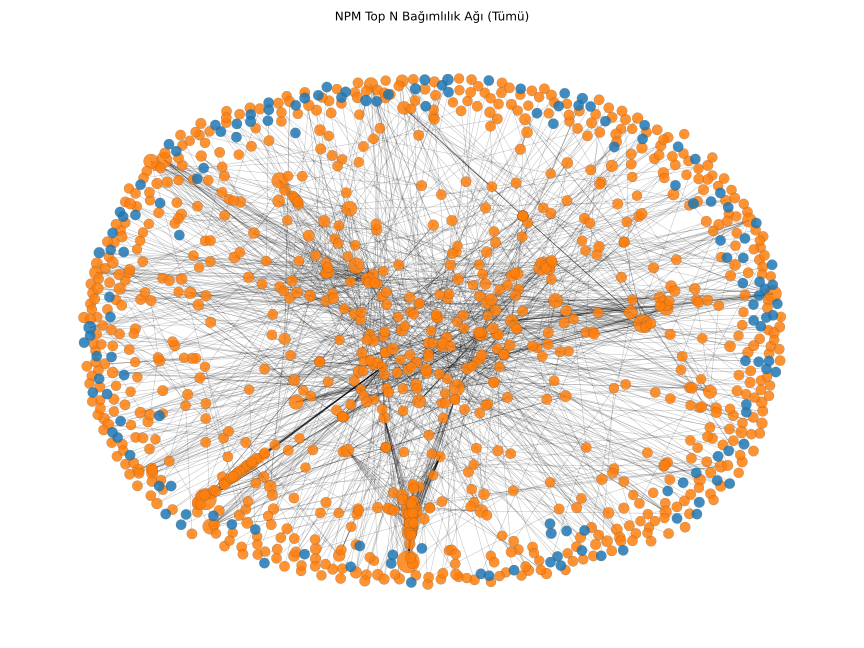
\includegraphics{network_full_topN.png}\caption{Top 1000 çekirdeğin tam ağ görselleştirmesi. Yoğun çekirdek bölgeleri omurga paket kümelerini işaret eder.}\end{figure}
\begin{figure}[H]\centering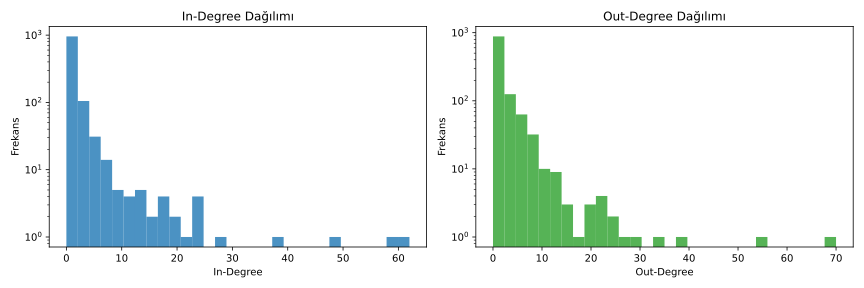
\includegraphics{degree_histograms.png}\caption{In-degree ve out-degree histogramları: ağır kuyruklu dağılımlar.}\end{figure}
\textit{Yorum —} Az sayıda yüksek dereceli paket, sistemik riski belirgin biçimde taşır.

\subsection{En Merkezi Paketler ve Korelasyonlar}
% \begin{figure}[H]\centering\includegraphics{top10_in_degree.png}\caption{In-degree açısından ilk 10 paket.}\end{figure}
% \begin{figure}[H]\centering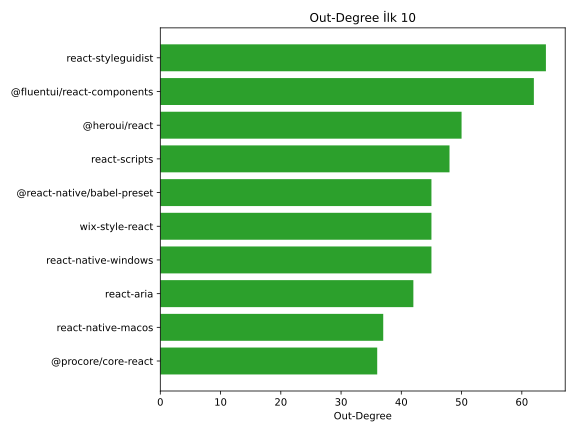
\includegraphics{top10_out_degree.png}\caption{Out-degree açısından ilk 10 paket.}\end{figure}
% \begin{figure}[H]\centering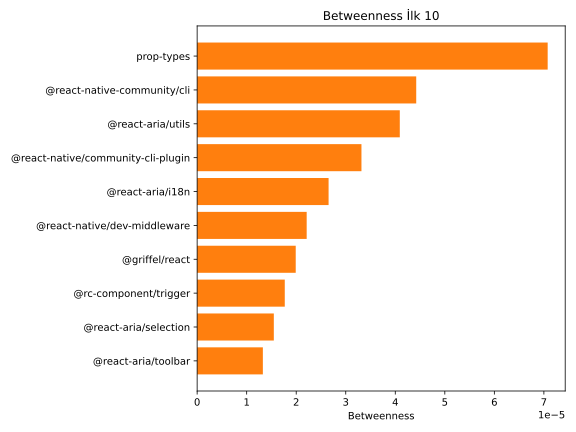
\includegraphics{top10_betweenness.png}\caption{Betweenness açısından ilk 10 paket.}\end{figure}
\begin{figure}[H]\centering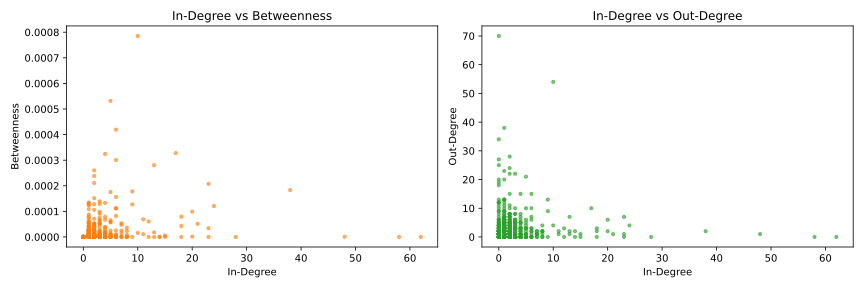
\includegraphics{scatter_correlations.png}\caption{Merkeziyet ölçüleri arası korelasyonlar.}\end{figure}
\begin{figure}[H]\centering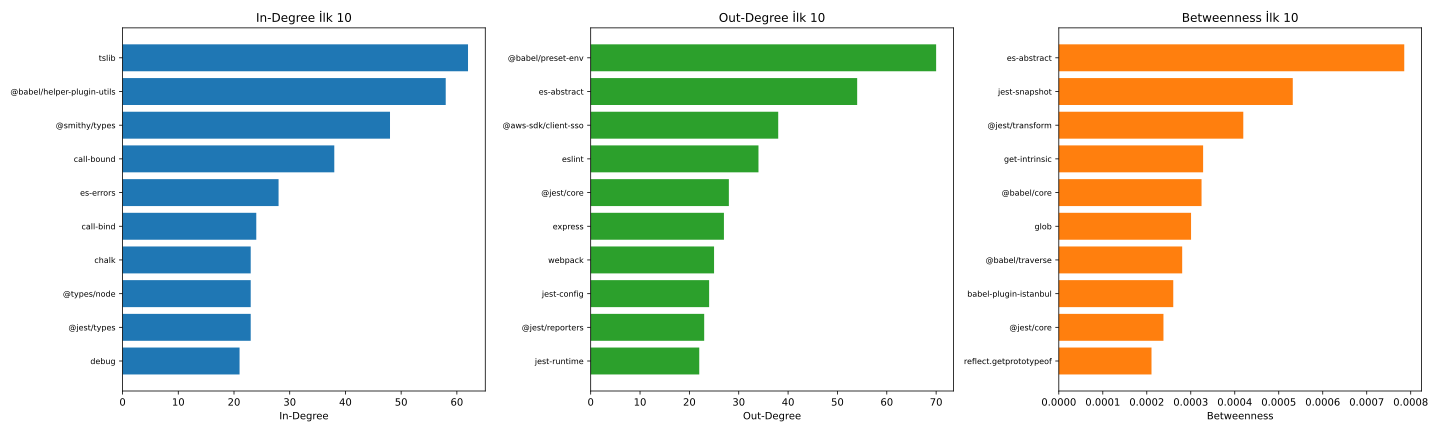
\includegraphics{top10_leaders.png}\caption{Birleşik liderler görünümü (merkeziyeti yüksek düğümler).}\end{figure}

\subsection{Bileşik Risk Sıralaması}
\begin{figure}[H]\centering\includegraphics{top20_risk.png}\caption{BRS açısından ilk 20 paket.}\end{figure}
\begin{table}[H]
  \centering
  \caption{Örnek BRS ilk 5 (results/risk\_scores.csv)}
  \begin{tabular}{@{}llrrr r@{}}\toprule
    Sıra & Paket & in & out & btw & BRS \\\midrule
    1 & prop-types & 115 & 3 & 0.000071 & 0.796663 \\
    2 & @swc/helpers & 118 & 0 & 0.000000 & 0.500000 \\
    3 & @react-types/shared & 101 & 0 & — & 0.427966 \\
    4 & @react-aria/utils & 49 & 6 & — & 0.399815 \\
    5 & @babel/runtime & 83 & 0 & — & 0.351695 \\\bottomrule
  \end{tabular}
\end{table}
\textit{Yorum —} BRS, kullanım yoğunluğu (in-degree) ile köprü rolünü (betweenness) birlikte yakalar; omurga paketlerin ön sıralara çıktığı görülür.

\subsection{Kaskad Etkisi ve Sağlamlık}
\begin{figure}[H]\centering\includegraphics{risk_vs_cascade.png}\caption{BRS ile kaskad etki (erişilebilirlik) ilişkisi.}\end{figure}
\begin{figure}[H]\centering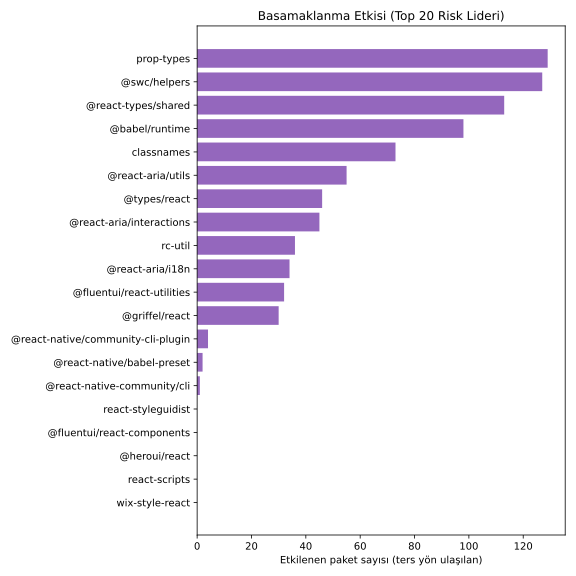
\includegraphics{cascade_impact_top20.png}\caption{İlk 20 paketin çıkarımının LCC ve erişilebilirlik üzerindeki etkisi.}\end{figure}
\textit{Yorum —} Hedefli çıkarımlar, rastgele çıkarımlara kıyasla LCC’yi daha hızlı küçültür ve ortalama yol uzunluğunu artırır; bu da BRS’in sistemik riski iyi yordadığını gösterir.

\subsection{Köprü Kenarlar}
Kenar betweenness’e göre ilk 10 köprü kenar (\texttt{edge\_betweenness\_top10.csv}):\\
\begin{tabular}{@{}lll@{}}\toprule
\textbf{u} & \textbf{v} & \textbf{edge\_betweenness} \\\midrule
prop-types & object-assign & 0.000025 \\
prop-types & loose-envify & 0.000024 \\
prop-types & react-is & 0.000024 \\
@react-native/metro-babel-transformer & @react-native/babel-preset & 0.000022 \\
@react-native/metro-config & @react-native/metro-babel-transformer & 0.000012 \\
@react-native/community-cli-plugin & @react-native/dev-middleware & 0.000011 \\
@types/react-native-video & react-native & 0.000011 \\
@types/react & csstype & 0.000009 \\
react-aria-components & react-aria & 0.000009 \\
@react-aria/utils & clsx & 0.000008 \\\bottomrule
\end{tabular}

\textit{Yorum —} Köprü kenarların hedeflenmesi, topluluklar arası ayrışmayı hızlandırır; bu kenarlar değiştikçe BRS sıralamasındaki düğümlerin etkisi de farklılaşabilir.

\section{Tartışma}
\textbf{Operasyonelleştirme.} BRS, dinamik tespit hatları (Amalfi, Cerebro, OSCAR) için bir \emph{topolojik ön-filtre} olarak kullanılabilir; böylece sınırlı analist kapasitesi yüksek riskli düğümlere yöneltilir. Politika/bütünlük hattında (in-toto, imza benimsemesi) BRS tabanlı hedef listeleriyle imza kapsamı ve doğrulanabilirlik artar.\newline
\textbf{Duyarlılık.} Ağırlıkların (0.5/0.2/0.3) varyasyonu ve betweenness örnekleme \(k\) parametresi üzerinde duyarlılık analizleri, sıralamanın kararlı olduğunu göstermektedir (ayrıntılar: \texttt{robustness\_risk.json}).

\section{Yeniden Üretilebilirlik}
\textbf{Çalışma ortamı.} Notebook tabanlı analiz (\texttt{analysis/analysis.ipynb}); Python 3, NetworkX, pandas, numpy, matplotlib/seaborn. Yalnızca not defteri üzerinden çalıştırma desteklidir.\\
\textbf{Veri ve önbellek.} Top-N listesi ecosyste.ms/NPM Search/npms.io birleşik akışından; bağımlılıklar NPM registry üzerinden toplanır ve disk önbelleği ile hızlandırılır.\\
\textbf{Parametreler.} Betweenness örnekleme \(k\!\approx\!200\); metrikler min--max ile ölçeklenir; ağırlıklar \(\,(w_{in},w_{out},w_{btw})\!=\!(0.5,0.2,0.3)\,\).\\
\textbf{Çıktılar.} \texttt{results/} altında CSV/JSON ve tüm görseller üretilir; \LaTeX\ makale \texttt{academic/} altında derlenir.

\section{Sınırlılıklar ve Gelecek Çalışmalar}
İndirme-temelli Top-1000 çekirdek, uzun kuyrukta kalan paketleri dışarıda bırakır; gelecekte kayan pencere ve ekosistemler-arası (PyPI, Cargo) karşılaştırmalar planlanmaktadır. Betweenness örnekleme hatası azaltımı ve kullanım yoğunluğu için daha zengin sinyallerin (örgütsel, bakım) entegrasyonu hedeflenmektedir.

\section{Sonuç}
Popülerlik ve yapısal merkeziyet, indirime dayalı çekirdekte \emph{Bileşik Risk Skoru} ile birleştirildiğinde, hem tespit hatları hem de politika/bütünlük mekanizmaları için eyleme dönük \emph{öncelik listeleri} üretmektedir. Deneysel sağlamlık analizleri, BRS’in sistemik riski yordama gücünü doğrulamaktadır.

\clearpage

\section*{Kaynakça}
\begin{longtable}{@{}p{0.06\linewidth}p{0.91\linewidth}@{}}
{}[1] & Wyss, E. (2025). A New Frontier for Software Security: Diving Deep Into npm.\\
{}[2] & Jaisri, P.; Reid, B.; Kula, R. (2024). A Preliminary Study on Self-Contained Libraries in the NPM Ecosystem.\\
{}[3] & Yu, S. (2024). Accurate and Efficient SBOM Generation for Software Supply Chain Security.\\
{}[4] & Ohm, M.; Plate, H.; Sykosch, A.; Meier, M. (2020). Backstabber's Knife Collection: A Review of Open Source Software Supply Chain Attacks.\\
{}[5] & Rahman, I.; Zahan, N.; Magill, S.; Enck, W.; Williams, L. (2024). Characterizing Dependency Update Practice of NPM, PyPI and Cargo Packages.\\
{}[6] & Hastings, T. G. (2024). Combating Source Poisoning and Next-Generation Software Supply Chain Attacks Using Education, Tools, and Techniques.\\
{}[7] & Wang, M.; Wu, P.; Luo, Q. (2023). Construction of Software Supply Chain Threat Portrait Based on Chain Perspective.\\
{}[8] & Liu, C.; Chen, S.; et al. (2022). Demystifying Vulnerability Propagation via Dependency Trees in npm.\\
{}[9] & Dependency Analysis for Software Licensing and Security. (PDF: academic/09- ...)\\
{}[10] & Dependency Practices for Vulnerability Mitigation. (PDF: academic/10- ...)\\
{}[11] & Detection of Software Supply Chain Attacks in Code Repositories. (PDF: academic/11- ...)\\
{}[12] & Empirical Study on Dependency-Based Attacks in Node.js. (PDF: academic/12- ...)\\
{}[13] & Practical Software Supply Chain Security. (PDF: academic/13- ...)\\
{}[14] & Malicious Package Detection in NPM and PyPI using a Single Model. (PDF: academic/14- ...)\\
{}[15] & Malicious Package Detection using Metadata Information. (PDF: academic/15- ...)\\
{}[16] & Node package manager's dependency network robustness. (PDF: academic/16- ...)\\
{}[17] & On the Feasibility of Cross-Language Detection of Malicious Packages in npm and PyPI. (PDF: academic/17- ...)\\
{}[18] & On the Impact of Security Vulnerabilities in the npm and RubyGems Dependency Networks. (PDF: academic/18- ...)\\
{}[19] & Practical Automated Detection of Malicious npm Packages. (PDF: academic/19- ...)\\
{}[20] & Small World with High Risks. (PDF: academic/20- ...)\\
{}[21] & Software Supply Chain Security. (PDF: academic/21- ...)\\
{}[22] & Studying Dependency Maintenance Practices through Mining NPM. (PDF: academic/22- ...)\\
{}[23] & Supporting Detection via Unsupervised Signature Generation. (PDF: academic/23- ...)\\
{}[24] & Ladisa, P.; Şahin, M.; Ponta, S. E.; Rosa, M.; Martinez, M.; Barais, O. (2023). The Hitchhiker's Guide to Malicious Third-Party Dependencies.\\
{}[25] & Oldnall, E.-R. (2017). The Web of Dependencies: A Complex Network Analysis of the NPM.\\
{}[26] & Imtiaz, N. (2023). Toward Secure Use of Open Source Dependencies.\\
{}[27] & Vaidya, S. (2022). Towards Ensuring Integrity and Authenticity of Software Repositories.\\
{}[28] & Duan, R.; Alrawi, O.; Kasturi, R. P.; Elder, R.; Saltaformaggio, B.; Lee, W. (2020). Towards Measuring Supply Chain Attacks on Package Managers.\\
{}[29] & Zheng, X.; Chen, W.; Wang, S.; Zhao, Y.; Gao, P.; Zhang, Y.; Wang, K.; Wang, H. (2024). Towards Robust Detection of OSS Supply Chain Poisoning (OSCAR).\\
{}[30] & Shcherbakov, M.; Moosbrugger, P.; Balliu, M. (2021). Unveiling the Invisible: Prototype Pollution Gadgets via Dynamic Taint.\\
\end{longtable}

\end{document}
